\chapter{Elementi caratterizzanti del progetto}
\label{cap:elementi-progetto}
% Qui introdurrò brevemente il contenuto delle sezioni sottostanti.
Questo capitolo si occupa di introdurre gli strumenti utilizzati nel corso del tirocinio, definire e dare una visione concreta delle attività di sviluppo del progetto di \textit{stage} e dare prova dei risultati raggiunti 
a livello di documentazione, di codice scritto, \textit{test coverage} e obiettivi raggiunti. 

\section{Stile lavorativo}

% In questa sezione descriverò il modo in cui ho lavorato nel corso del tirocinio, descrivendo attività esterne allo sviluppo, alla verifica ed alla validazione e descrivendo il modo in cui invece tali attività sono state ideate.
Data la pianificazione a cadenza settimanale delle attività (sezione \hyperref[sec:pianificazione]{§2.5}), ho concordato con il tutor aziendale, il signor \textit{Michele Rigo}, l'organizzazione di una riunione di allineamento settimanale, programmata per ogni lunedì mattina. \\
Tale incontro mirava a:
\begin{itemize}
    \item Mostrare il lavoro svolto nel corso della settimana precedente alla riunione;
    \item Condurre una retrospettiva sulla settimana precedente;
    \item Valutare lo stato di avanzamento del progetto in relazione alle aspettative;
    \item Delineare le attività da svolgere nella settimana in corso.
\end{itemize}

\begin{figure}[H]
    \centering
    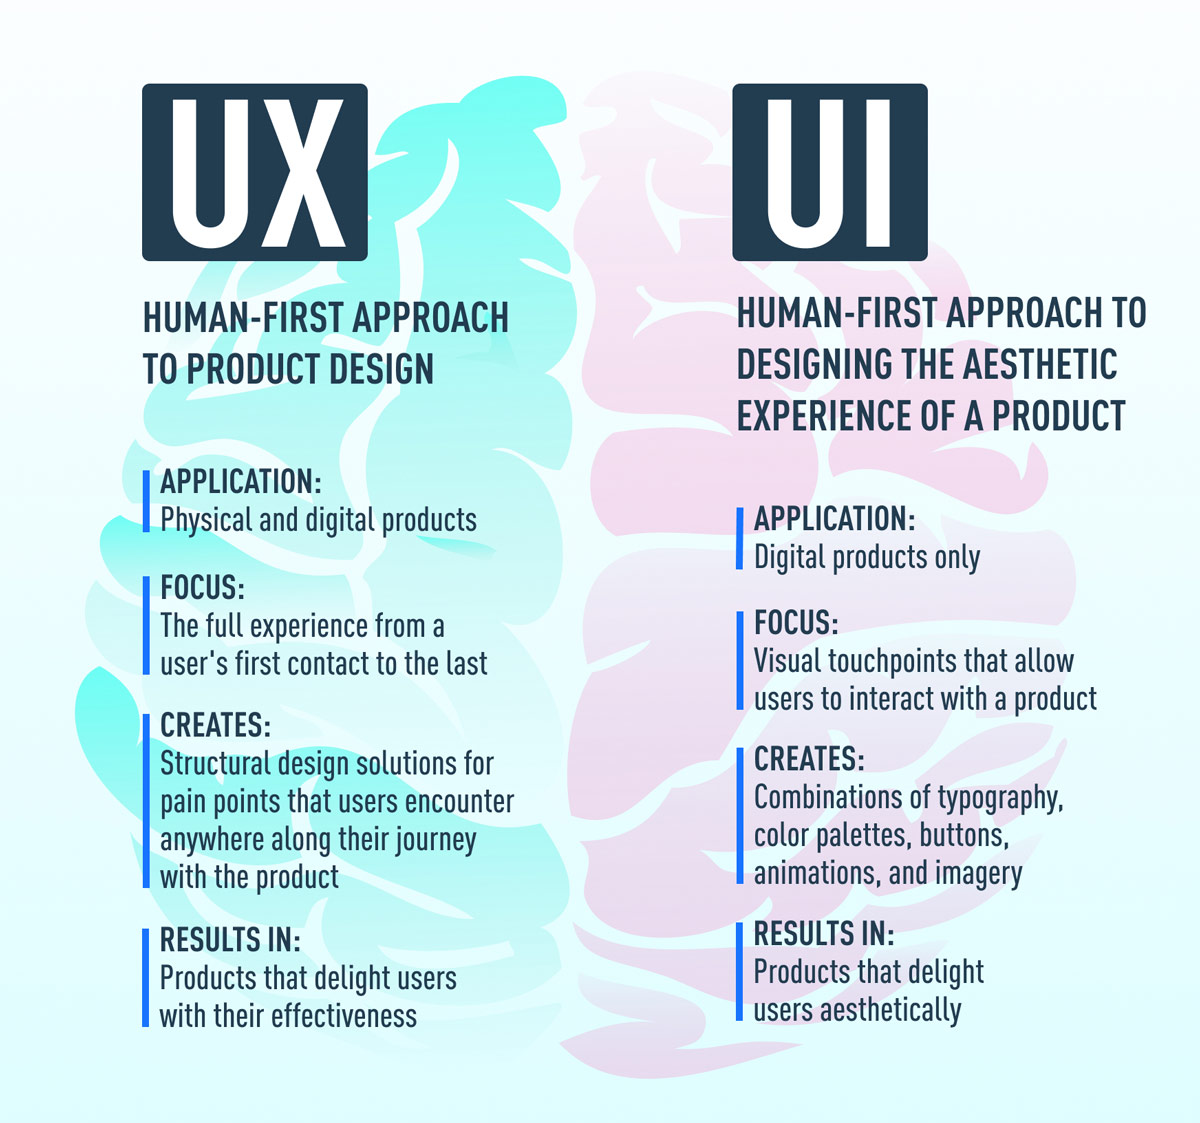
\includegraphics[width=0.8\textwidth]{images/difference-between-ux-and-ui.jpg}
    \caption[Confronto tra la progettazione di interfacce e di esperienze utente]{Confronto tra la progettazione di interfacce (\textit{UI, User Interface}) e di esperienze utente (\textit{UX, User Experience})\footnotemark}
\end{figure}
\footnotetext{Fonte: \href{https://careerfoundry.com/en/blog/ux-design/the-difference-between-ux-and-ui-design-a-laymans-guide/}{https://careerfoundry.com}}
Abbiamo svolto degli incontri aggiuntivi in forma telematica per chiarire alcuni aspetti del progetto, in particolare la comprensione di alcuni requisiti utente e la definizione di determinati aspetti 
di interfaccia grafica ed esperienza utente (ovvero come l'utente può interagire con l'interfaccia grafica, la relazione che intercorre tra egli e gli elementi grafici). \\
Per tutta la durata delle attività di \textit{stage}, sono stato affiancato in caso di necessità da praticamente tutto il \textit{team \textbf{Trizeta}}, soprattutto per quanto concerne la progettazione dell'interfaccia grafica.

% \newline

% Le attività di sviluppo del prodotto hanno seguito le specifiche del \textbf{modello a V}, ovvero:
% \begin{figure}[H]
%     \centering
%     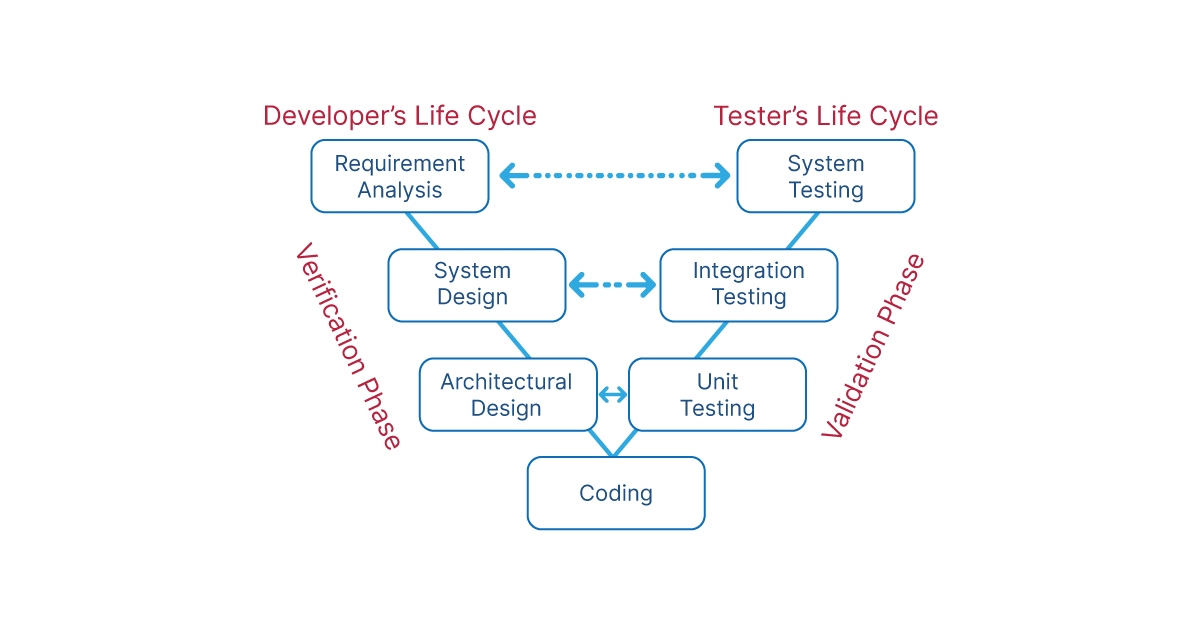
\includegraphics[width=\textwidth]{images/v-model.jpg}
%     \caption[Modello di sviluppo del prodotto adottato]{Modello di sviluppo del prodotto adottato\footnotemark}
% \end{figure}
% \footnotetext{Fonte: \href{https://www.shiksha.com/online-courses/articles/v-model-software-engineering/}{https://www.shiksha.com}}

\section{Strumenti utilizzati}
% In questa sezione descriverò gli strumenti utilizzati nel corso del progetto, suddividendoli in base alle attività in cui essi sono stati impiegati.

\subsection{Strumenti di sviluppo}
    \subsubsection*{Angular}
        \begin{itemize}
            \item [\textit{Versione}:] 16.2.9
            \item [\textit{Descrizione}:] è un \textit{framework open-source} per lo sviluppo di applicazioni \textit{web} a singola pagina (è un tipo di applicazione \textit{web} che opera all'interno di una singola pagina \textit{web}, senza la necessità di ricaricarla durante l'interazione dell'utente). \\ 
                    Sviluppato da \textit{Google}, \textit{Angular} fornisce una struttura per la costruzione di applicazioni \textit{web} che consentono agli sviluppatori di utilizzare il linguaggio \textit{TypeScript} o \textit{JavaScript} per la creazione di componenti riutilizzabili.
        \end{itemize}
    \subsubsection*{Angular Material}
    \begin{itemize}
        \item [\textit{Versione}:] 16.2.8
        \item [\textit{Descrizione}:] è una libreria di componenti grafiche e direttive, sviluppata da \textit{Google} e progettata per essere utilizzata con il \textit{framework Angular}. \\
                     Questa libreria fornisce una serie di componenti predefiniti e stilizzati che semplificano la creazione di interfacce utente coerenti e moderne all'interno delle applicazioni \textit{Angular}.
    \end{itemize}

    \subsubsection*{Figma}
    \begin{itemize}
        \item [\textit{Versione}:] 9.0
        \item [\textit{Descrizione}:] è un'applicazione di progettazione e prototipazione basata su \textit{cloud} (\textit{software} il cui funzionamento e archiviazione dei dati avvengono prevalentemente attraverso risorse di calcolo e archiviazione disponibili su \textit{Internet}, anziché su risorse locali o \textit{server} fisici) 
                    che consente di collaborare in tempo reale su progetti di interfaccia utente (\textit{UI}) ed esperienza utente (\textit{UX}).
    \end{itemize}

    \subsubsection*{Karma}
    \begin{itemize}
        \item [\textit{Versione}:] 6.4.0
        \item [\textit{Descrizione}:] è uno strumento ampiamente utilizzato per l'esecuzione di \textit{test} di unità per applicazioni \textit{Angular}. \\
                    \textit{Karma} genera un \textit{server web} che esegue il codice di \textit{test Javascript} (e \textit{TypeScript}, che ne è sovralinguaggio) per ogni \textit{browser} connesso.
    \end{itemize}

    \subsubsection*{Node.js}
    \begin{itemize}
        \item [\textit{Versione}:] 18.17.1
        \item [\textit{Descrizione}:] è un ambiente di \textit{runtime open source} basato sul motore \textit{JavaScript} V8 di \textit{Google Chrome}. \\
                    Consente di eseguire codice \textit{JavaScript} lato \textit{server}, dando l'opportunità agli sviluppatori di utilizzare \textit{JavaScript} per lo sviluppo di applicazioni \textit{back-end}.
    \end{itemize}

    \subsubsection*{Ng-openapi-gen}
    \begin{itemize}
        \item [\textit{Versione}:] 0.50.2
        \item [\textit{Descrizione}:] è un modulo \textit{npm} (il gestore di pacchetti per \textit{Node.js}) che genera servizi, 
                    modelli e funzioni \textit{Angular} a partire da una specifica \textit{OpenAPI 3} (è uno \textit{standard} che aiuta a descrivere e documentare le Interfacce di Programmazione delle Applicazioni, \glslink{apig}{\textit{API}}).
    \end{itemize}

    \subsubsection*{Ngx-translate}
    \begin{itemize}
        \item [\textit{Versione}:] 15.0.0
        \item [\textit{Descrizione}:] libreria che consente l'internazionalizzazione (ovvero facilita l'astrazione del contenuto statico di un'applicazione \textit{web} rispetto alla lingua di fruizione) e la localizzazione (ovvero consente di adattare il \textit{software} in base alle esigenze culturali dell'area in cui il prodotto viene usato) in \textit{Angular}.
    \end{itemize}

    \subsubsection*{StarUML}
    \begin{itemize}
        \item [\textit{Versione}:] 6.0.1
        \item [\textit{Descrizione}:] è uno strumento di modellazione \textit{UML}\footnote{\glslink{umlg}{\textit{Unified Modeling Language}}} (\textit{Unified Modeling Language}) che offre un ambiente grafico per progettare e visualizzare diagrammi \glslink{umlg}{\textit{UML}}. \\
                \glslink{umlg}{\textit{UML}} è uno \textit{standard} per la modellazione visuale di sistemi \textit{software}, ed è utilizzato per rappresentare graficamente diversi aspetti di un sistema come le classi, i casi d'uso, le sequenze di chiamate, le attività, e altro ancora.
    \end{itemize}

    \subsubsection*{TypeScript}
    \begin{itemize}
        \item [\textit{Versione}:] 5.1.6
        \item [\textit{Descrizione}:] è un linguaggio di programmazione \textit{open-source} sviluppato da \textit{Microsoft}. \\
                È una versione "\textit{superset}" di \textit{JavaScript}, il che significa che aggiunge nuove funzionalità e tipizzazione statica al linguaggio JavaScript.
    \end{itemize}

    \subsubsection*{Visual Studio Code}
    \begin{itemize}
        \item [\textit{Versione}:] 1.84.1
        \item [\textit{Descrizione}:] è un \textit{editor} di codice sorgente gratuito e \textit{open-source} sviluppato da \textit{Microsoft}. \\
                È progettato per essere leggero, flessibile e altamente personalizzabile, rendendolo uno strumento popolare tra gli sviluppatori per la scrittura di codice in diversi linguaggi di programmazione.
    \end{itemize}


\subsection{Strumenti di versionamento}
    \subsubsection*{Git}
    \begin{itemize}
        \item [\textit{Versione}:] 2.43.0
        \item [\textit{Descrizione}:] è un sistema di controllo delle versioni distribuito (\textit{DVCS, Distributed Version Control System}), utilizzato per tracciare le modifiche apportate al codice sorgente durante lo sviluppo del \textit{software}.
    \end{itemize}

    \subsubsection*{GitHub}
    \begin{itemize}
        \item [\textit{Versione}:] 3.11.0
        \item [\textit{Descrizione}:] è una piattaforma di \textit{hosting} per il controllo delle versioni e la collaborazione. \\
                    Offre servizi basati su \textit{Git} e facilita la gestione e la condivisione dei progetti \textit{software}.
    \end{itemize}

\subsection{Strumenti di documentazione}

\subsubsection*{Compodoc}
\begin{itemize}
    \item [\textit{Versione}:] 1.1.22
    \item [\textit{Descrizione}:] strumento \textit{open-source} per la generazione di documentazione per \textit{web app Angular} a partire da commenti scritti nel codice sorgente.
\end{itemize}

\subsubsection*{LibreOffice}
\begin{itemize}
    \item [\textit{Versione}:] 7.6.2
    \item [\textit{Descrizione}:] è una \textit{suite} di \textit{software} per l'ufficio libera e \textit{open-source} che offre un insieme di applicazioni per la produttività personale e professionale. \\
                È sviluppato dalla comunità di sviluppatori di \textit{The Document Foundation} ed è una delle alternative più popolari e complete a \textit{suite} di produttività come \textit{Microsoft Office}.
\end{itemize}

\section{Analisi dei requisiti}
% In questa sezione descriverò lo scopo dell'analisi dei requisiti in un progetto, le problematiche riscontrate e mostrerò i principali casi d'uso ed i principali requisiti elaborati.
Le attività di \textbf{analisi dei requisiti} hanno come scopo la comprensione dei bisogni espressi dall'utente finale, detti "requisiti utente" (o da chi vuole risolvere tali bisogni all'utente finale, talvolta nemmeno noti all'utente finale \footnote{Fonte: \href{https://www.mountaingoatsoftware.com/articles/i-didnt-know-i-needed-that}{https://www.mountaingoatsoftware.com}}) 
e la definizione di "ciò che deve svolgere il prodotto" per soddisfare tali bisogni, detti "requisiti del prodotto". \\
Ho iniziato le attività di analisi con un incontro sincrono, insieme al tutor aziendale, relativo all'infrastruttura aziendale esistente (contesto delle attività produttive) e al ruolo che il prodotto da sviluppare (di nome \textit{ADeQA}) ricopre in questo contesto. \\
La contestualizzazione delle mie attività di \textit{stage} è stata seguita da una spiegazione dei bisogni da soddisfare: sono stati necessari più passi di raffinazione (descritti in seguito) dei bisogni espressi per arrivare a definire i requisiti del prodotto.

\subsection{Casi d'uso}
Con "caso d'uso" si intende un'astrazione utilizzata per catturare, descrivere e definire le interazioni tra un prodotto e gli attori (utenti o altri \textit{software}) che interagiscono con esso. \\
Un caso d'uso è una rappresentazione (narrativa e/o schematica) di uno scenario che descrive come il sistema risponde alle richieste degli utenti in determinate circostanze. \\
I casi d’uso qui presenti mirano a dare comprensione dei requisiti utente principali, pertanto non vengono riportati tutti i casi d'uso identificati in sede di \textit{stage}.
\subsubsection*{Nomenclatura}
 
I casi d'uso sono identificati da una sigla alfanumerica così composta:
\begin{center}
    \textbf{UC[Tipologia]-[Codice]}
\end{center}

\begin{itemize}
    \item \textbf{UC}: abbreviativo di "\textit{Use Case}";
    \item \textbf{Tipologia}: tipologia del caso d'uso:
        \begin{itemize}
            \item \textbf{F}: funzionale, descrive una funzionalità;
            \item \textbf{E}: errore, descrive cosa deve accadere in caso di un determinato errore.
        \end{itemize}
    \item \textbf{Codice}: identificativo numerico del caso d’uso, può identificare dei sotto-casi d’uso / generalizzazioni qualora si presentasse in forma \textbf{[caso].[identificativo]}.
\end{itemize}

\subsubsection*{Attori primari}
L’applicazione presenta due attori primari, ovvero due tipologie di utente finale:
\begin{itemize}
    \item \textbf{Utente non autenticato}: utente che non ha ancora effettuato l’autenticazione, avrà funzionalità limitate rispetto ad un utente autenticato;
    \item \textbf{Utente autenticato}: utente che ha effettuato l’autenticazione alla piattaforma tramite le proprie credenziali (nome utente, password e pin); ha accesso ad ogni funzionalità messa a disposizione.
\end{itemize}

\label{subsubsec:casi-d'uso}
\subsubsection*{Lista dei principali casi d'uso}
    \textbf{UCF-2: Visualizzazione delle fasi}
        \begin{figure}[H]
            \centering
            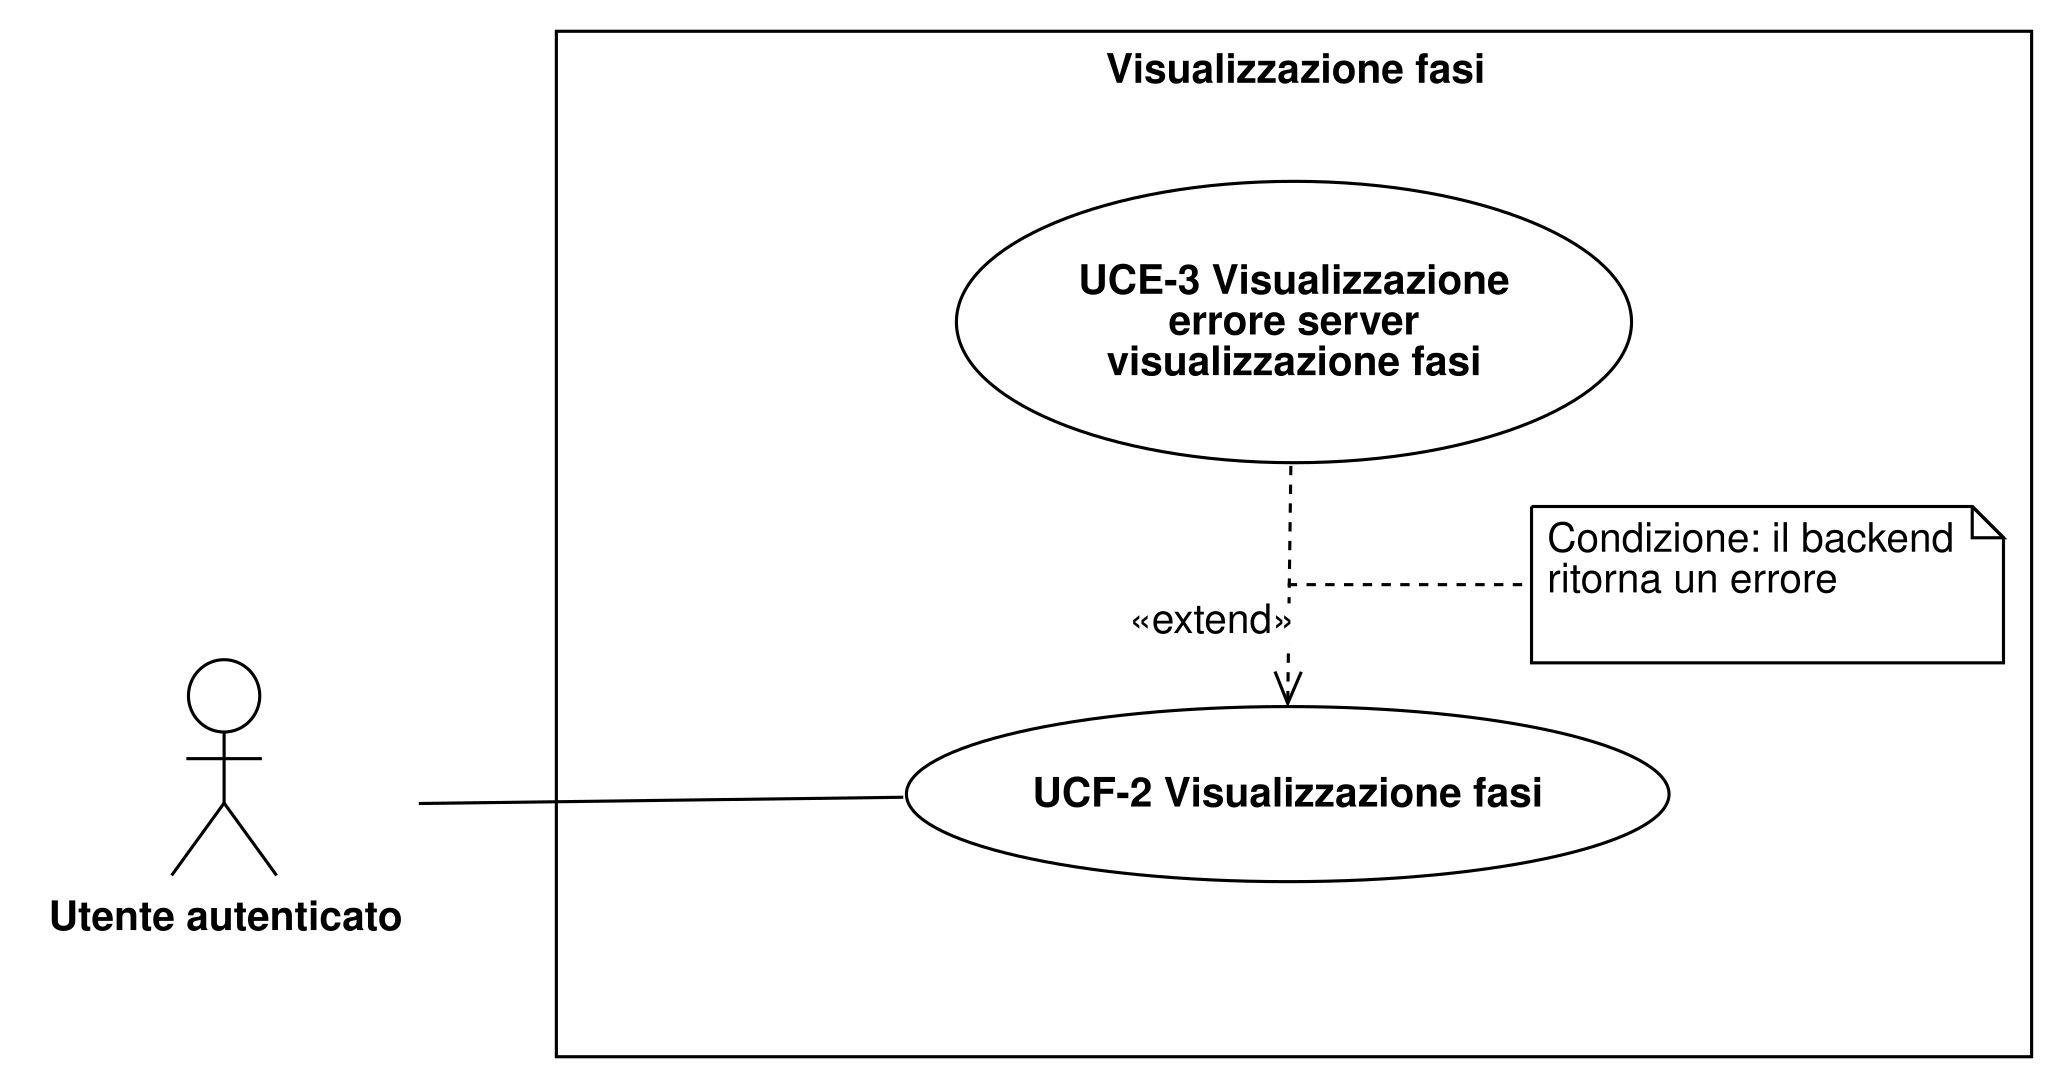
\includegraphics[width=0.9\textwidth]{usecase/UCF-2.png}
            \caption{Diagramma dei casi d'uso UCF-2 e UCE-3.}
        \end{figure}
        \begin{itemize}
            \item \textbf{Descrizione:} l’utente vuole visualizzare le fasi di lavorazione della filiera produttiva;
            \item \textbf{Scenario:}
                \begin{enumerate}
                    \item L’utente visualizza le fasi di lavorazione.
                \end{enumerate}
            \item \textbf{Estensioni:} si presenta un errore lato server alla lettura delle fasi di produzione (\textbf{UCE-3});
            \item \textbf{Attore principale:} utente autenticato;
            \item \textbf{Precondizioni:} l’utente è autenticato;
            \item \textbf{Postcondizioni:} l’utente visualizza le fasi di produzione.
        \end{itemize}

        \textbf{UCF-4: Visualizzazione degli attributi}
        \begin{figure}[H]
            \centering
            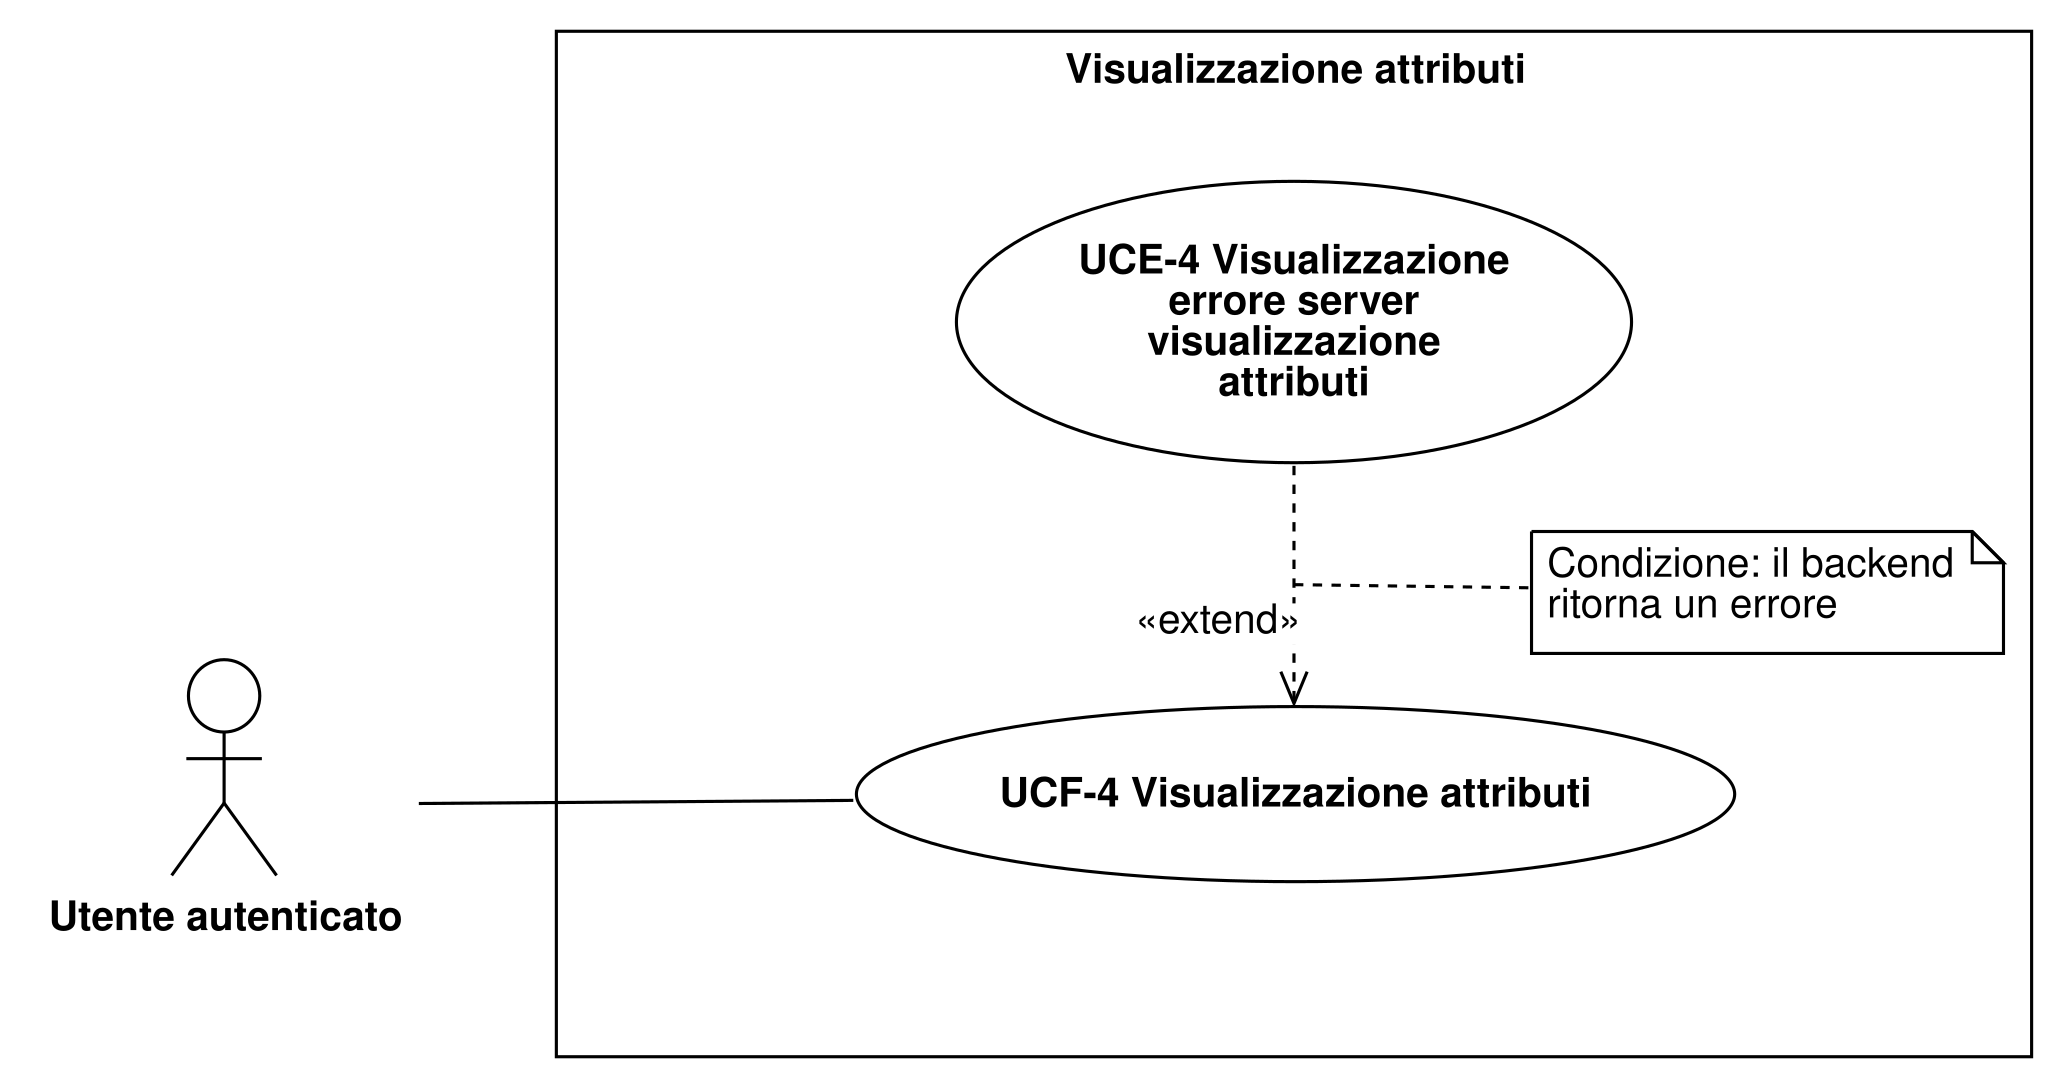
\includegraphics[width=0.9\textwidth]{usecase/UCF-4.png}
            \caption{Diagramma dei casi d'uso UCF-4 e UCE-4.}
        \end{figure}
        \begin{itemize}
            \item \textbf{Descrizione:} l’utente vuole visualizzare gli attributi della fase di lavorazione selezionata;
            \item \textbf{Scenario:}
                \begin{enumerate}
                    \item L’utente sta visualizzando le fasi di lavorazione;
                    \item L’utente seleziona una fase di lavorazione.
                \end{enumerate}
            \item \textbf{Estensioni:} si presenta un errore lato server alla lettura degli attributi della fase di produzione selezionata (\textbf{UCE-4});
            \item \textbf{Attore principale:} utente autenticato;
            \item \textbf{Precondizioni:} l’utente sta visualizzando le fasi di produzione;
            \item \textbf{Postcondizioni:} l’utente visualizza gli attributi della fase di produzione che ha selezionato.
        \end{itemize}


        \textbf{UCF-5: Valorizzazione degli attributi}
        \begin{figure}[H]
            \centering
            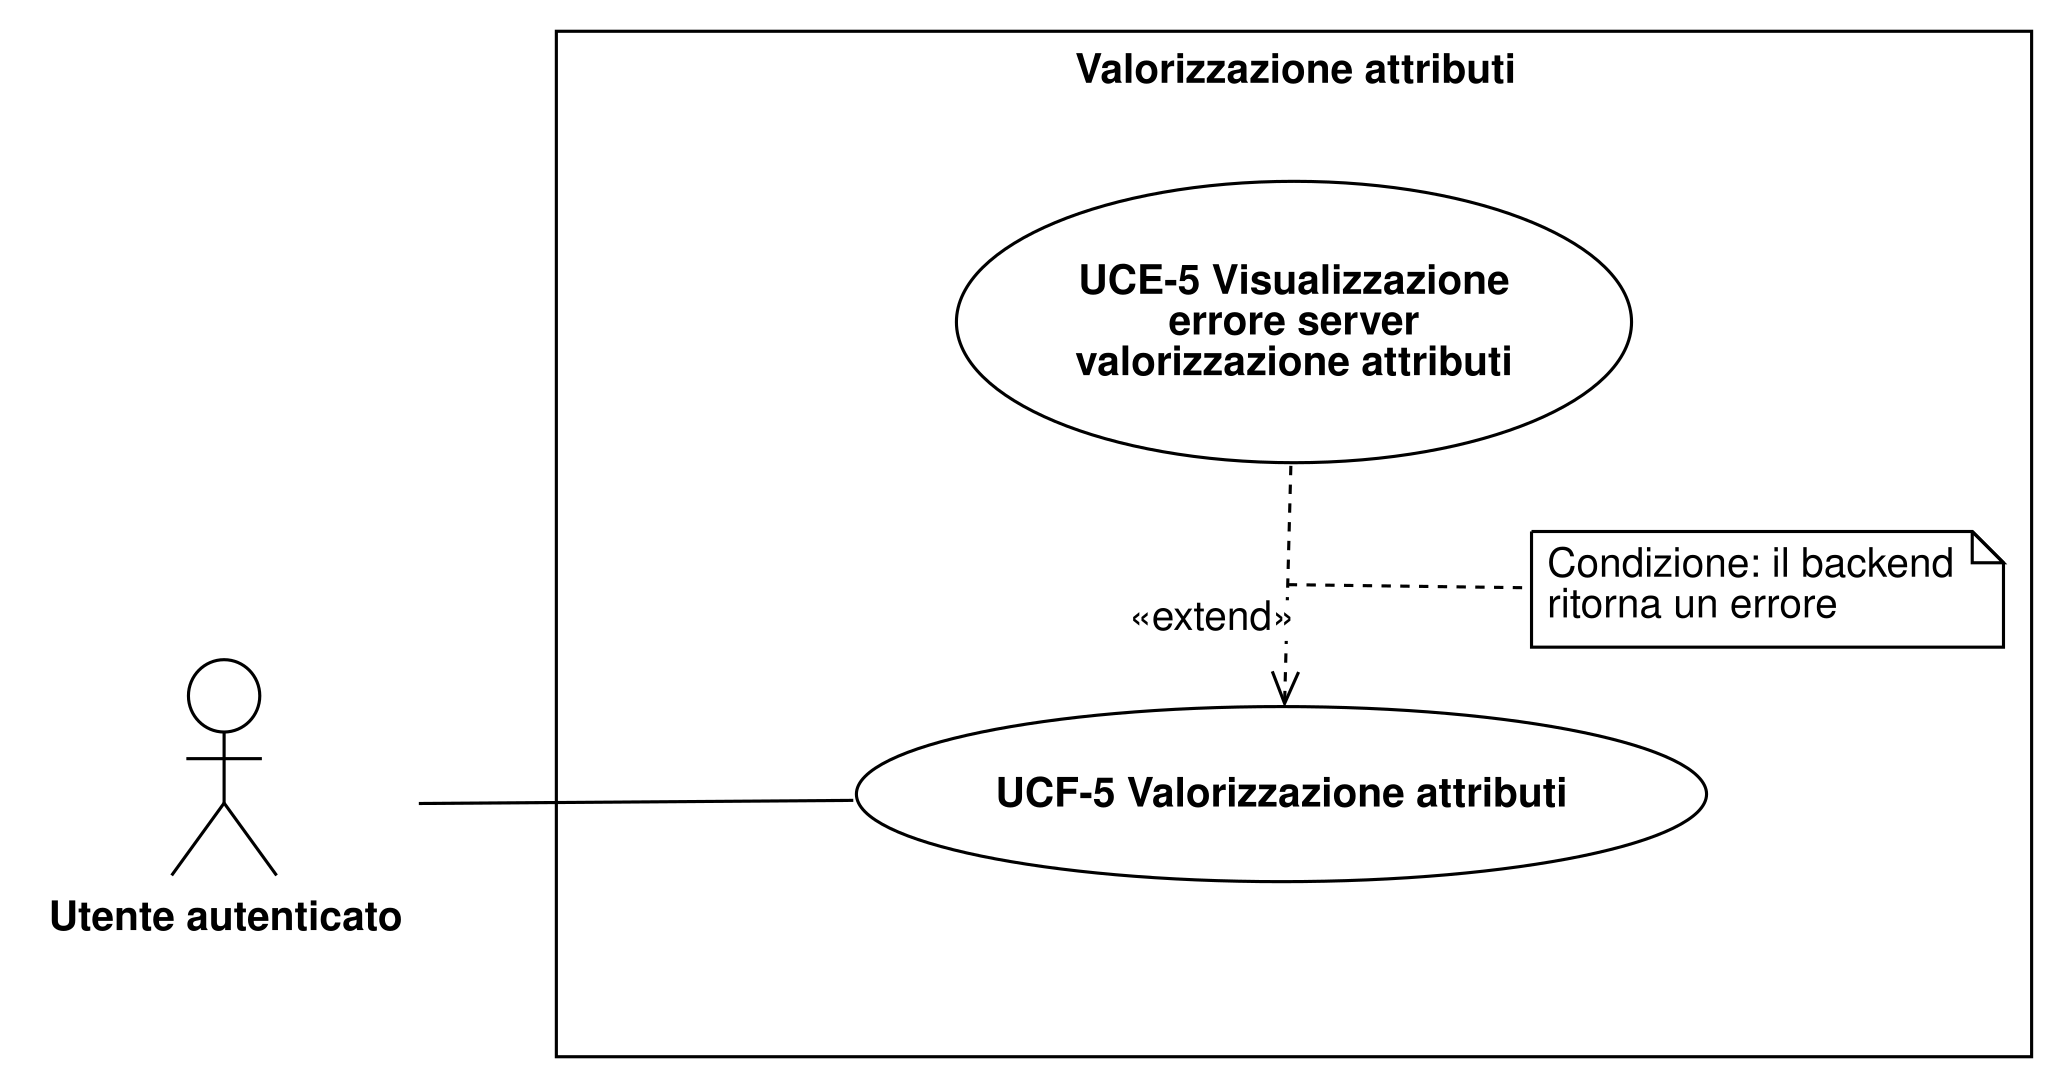
\includegraphics[width=0.9\textwidth]{usecase/UCF-5.png}
            \caption{Diagramma dei casi d'uso UCF-5 e UCE-5.}
        \end{figure}
        \begin{itemize}
            \item \textbf{Descrizione:} l’utente vuole inserire manualmente un valore per gli attributi della fase di lavorazione selezionata, creando un \textit{log} di controllo qualità;
            \item \textbf{Scenario:}
                \begin{enumerate}
                    \item L’utente visualizza gli attributi della fase di lavorazione selezionata;
                    \item L'utente assegna un valore agli attributi visualizzati;
                    \item L'utente conferma la scelta.
                \end{enumerate}
            \item \textbf{Estensioni:} si presenta un errore lato server all’inserimento del valore degli attributi della fase di produzione selezionata (\textbf{UCE-5});
            \item \textbf{Attore principale:} utente autenticato;
            \item \textbf{Precondizioni:} l’utente sta visualizzando gli attributi (\textbf{UCF-4});
            \item \textbf{Postcondizioni:} l’utente assegna un valore agli attributi di una fase di produzione che ha selezionato.
        \end{itemize}


        \textbf{UCF-7: Visualizzazione dei dati di qualità registrati}
        \begin{figure}[H]
            \centering
            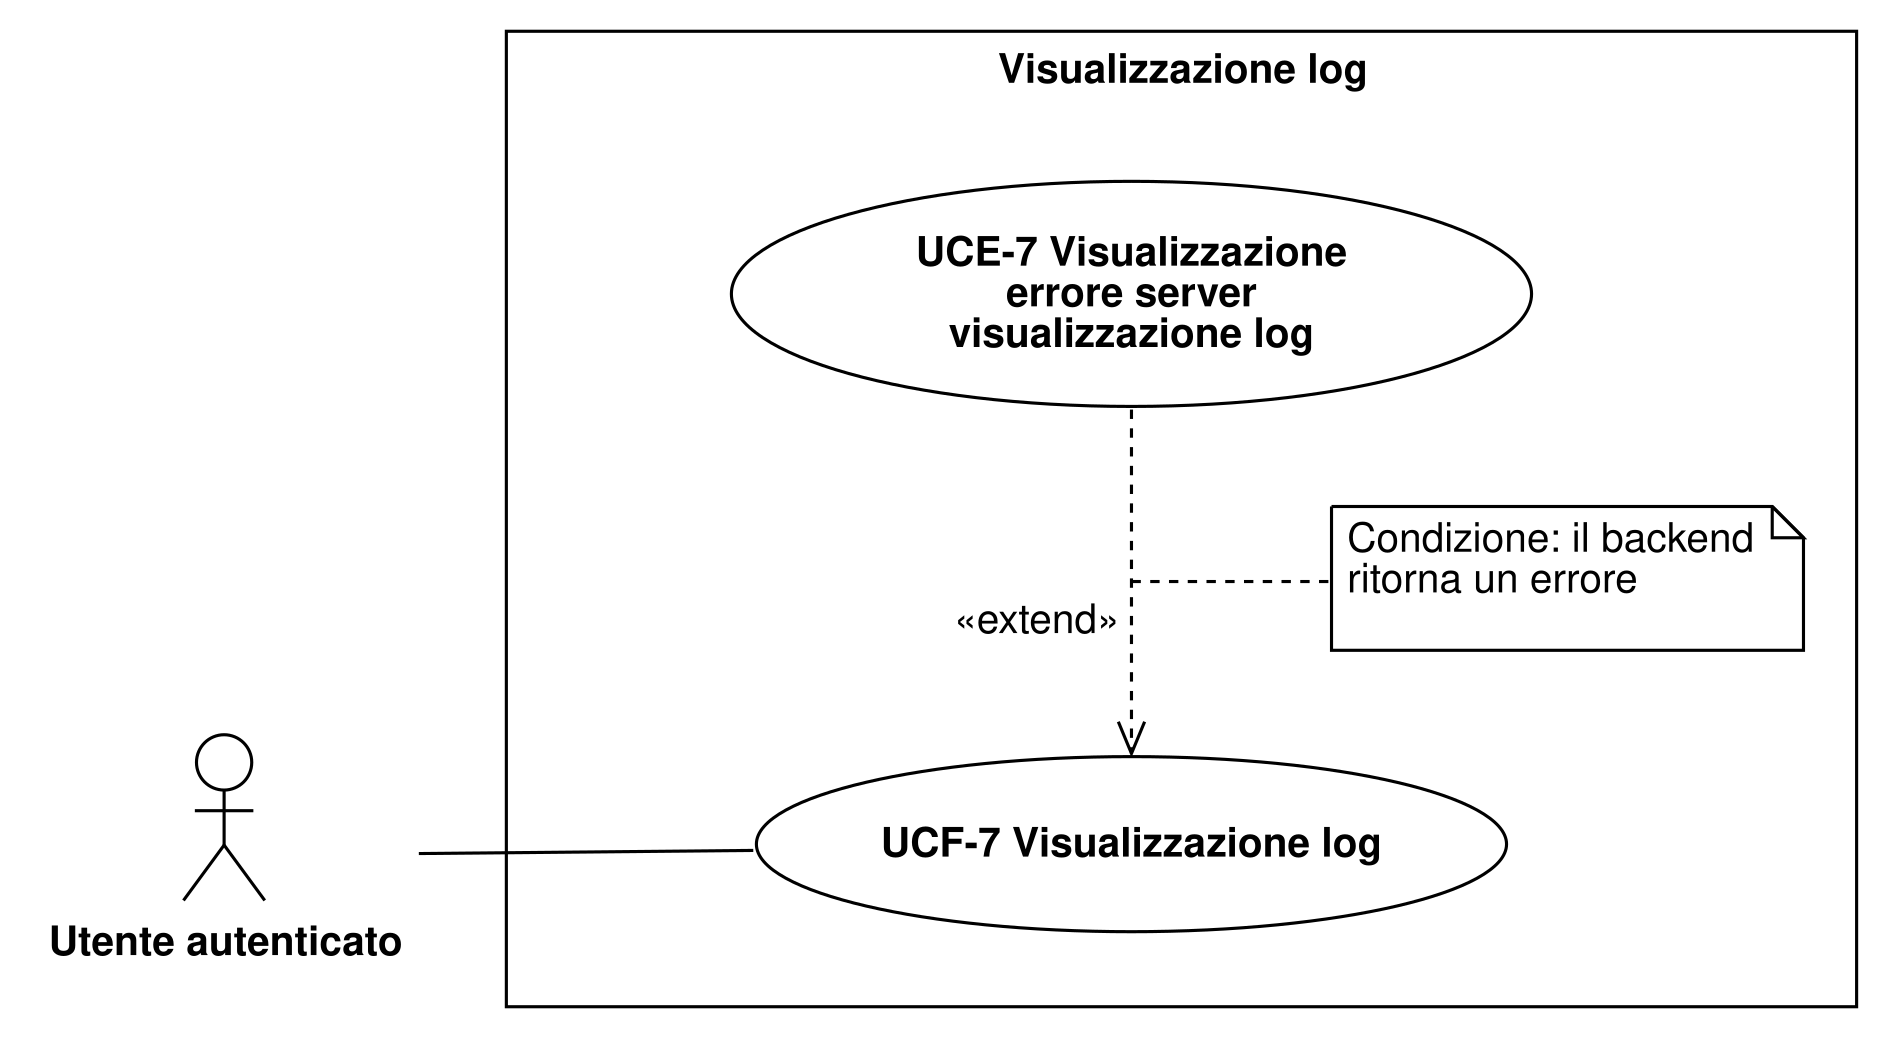
\includegraphics[width=0.9\textwidth]{usecase/UCF-7.png}
            \caption{Diagramma dei casi d'uso UCF-7 e UCE-7.}
        \end{figure}
        \begin{itemize}
            \item \textbf{Descrizione:} l’utente vuole visualizzare i dati di controllo qualità inseriti;
            \item \textbf{Scenario:}
                \begin{enumerate}
                    \item L’utente seleziona una fase di produzione;
                    \item L’utente visualizza i \textit{log} per la fase selezionata.
                \end{enumerate}
            \item \textbf{Estensioni:} si presenta un errore lato server durante il tentativo di acquisire i log di controllo qualità (\textbf{UCE-7});
            \item \textbf{Attore principale:} utente autenticato;
            \item \textbf{Precondizioni:} l’utente è autenticato;
            \item \textbf{Postcondizioni:} l’utente visualizza i dati di controllo qualità inseriti per la fase selezionata.
        \end{itemize}

        \textbf{UCE-3: Visualizzazione errore lato \textit{server} all’acquisizione delle fasi di lavorazione}
        \begin{itemize}
            \item \textbf{Descrizione:} l’utente vuole visualizzare le fasi di lavorazione e il \textit{server} ritorna un errore;
            \item \textbf{Scenario:}
                \begin{enumerate}
                    \item L’utente visualizza un messaggio di errore.
                \end{enumerate}
            \item \textbf{Attore principale:} utente autenticato;
            \item \textbf{Precondizioni:} l’utente vuole visualizzare le fasi di lavorazione (\textbf{UCF-2});
            \item \textbf{Postcondizioni:} l’utente visualizza un messaggio di errore relativo all’avvenimento di un errore lato \textit{server} all’acquisizione delle fasi di lavorazione.
        \end{itemize}

        \textbf{UCE-4: Visualizzazione errore lato \textit{server} all’acquisizione degli attributi delle fasi di lavorazione}
        \begin{itemize}
            \item \textbf{Descrizione:} l’utente vuole visualizzare gli attributi delle fasi di lavorazione e il \textit{server} ritorna un errore;
            \item \textbf{Scenario:}
                \begin{enumerate}
                    \item L’utente visualizza un messaggio di errore.
                \end{enumerate}
            \item \textbf{Attore principale:} utente autenticato;
            \item \textbf{Precondizioni:} l’utente vuole visualizzare le fasi di lavorazione (\textbf{UCF-2});
            \item \textbf{Postcondizioni:} l’utente visualizza un messaggio di errore relativo all’avvenimento di un errore lato \textit{server} all’acquisizione delle fasi di lavorazione.
        \end{itemize}

        \textbf{UCE-5: Visualizzazione errore lato \textit{server} alla valorizzazione degli attributi delle fasi di lavorazione}
        \begin{itemize}
            \item \textbf{Descrizione:} l’utente vuole assegnare un valore agli attributi della fase di lavorazione selezionata e il \textit{server} ritorna un errore;
            \item \textbf{Scenario:}
                \begin{enumerate}
                    \item L’utente visualizza un messaggio di errore.
                \end{enumerate}
            \item \textbf{Attore principale:} utente autenticato;
            \item \textbf{Precondizioni:} l’utente vuole assegnare un valore agli attributi della fase di lavorazione selezionata (\textbf{UCF-5});
            \item \textbf{Postcondizioni:} l’utente visualizza un messaggio di errore relativo all’avvenimento di un errore lato \textit{server} all’assegnazione di un valore agli attributi della fase di lavorazione selezionata.
        \end{itemize}

        \textbf{UCE-7: Visualizzazione errore lato \textit{server} all’acquisizione dei dati di controllo qualità}
        \begin{itemize}
            \item \textbf{Descrizione:} l’utente vuole visualizzare i \textit{log} di controllo qualità per la fase selezionata;
            \item \textbf{Scenario:}
                \begin{enumerate}
                    \item L’utente visualizza un messaggio di errore.
                \end{enumerate}
            \item \textbf{Attore principale:} utente autenticato;
            \item \textbf{Precondizioni:} l’utente vuole visualizzare i dati di controllo qualità per la fase selezionata (\textbf{UCF-7});
            \item \textbf{Postcondizioni:} l’utente visualizza un messaggio di errore relativo all’avvenimento di un errore lato \textit{server} alla visualizzazione dei dati di controllo qualità.
        \end{itemize}

\subsection{Requisiti}

Con "requisito" si intende una specifica di ciò che un sistema software deve fare o possedere al fine di soddisfare un determinato obiettivo o risolvere un particolare problema; i requisiti sono le basi per la progettazione, lo sviluppo e la verifica di un \textit{software}. \\
La lista di requisiti sotto riportata, a differenza della lista dei casi d'uso, è completa: serve per dare una visione completa del lavoro di analisi e offrire una base per la comprensione degli esempi di progettazione e codifica. \\
I casi d'uso \textit{UCF-2}, \textit{UCF-4}, \textit{UCF-5} e \textit{UCF-7} sono associati rispettivamente ai requisiti \textit{RF-2}, \textit{RF-4}, \textit{RF-5} e \textit{RF-7} della tabella dei \hyperref[tab:requisiti-funzionali]{requisiti funzionali}.
\subsubsection*{Nomenclatura}
 
I requisiti qui presenti sono identificati da una sigla alfanumerica così composta:
\begin{center}
    \textbf{R[Tipologia]-[Codice]}
\end{center}

\begin{itemize}
    \item \textbf{R}: abbreviativo di "requisito";
    \item \textbf{Tipologia}: tipologia del requisito:
        \begin{itemize}
            \item \textbf{F}: funzionale, descrive una funzionalità (ciò che un prodotto consente di fare all'utente);
            \item \textbf{Q}: di qualità, indica una caratteristica delle modalità di sviluppo;
            \item \textbf{P}: prestazionale, indica alcune caratteristiche che il prodotto deve avere durante l'esecuzione (non ciò che consente di fare);
            \item \textbf{V}: di vincolo, ovvero riguardante una caratteristica del prodotto stabilita prima del suo sviluppo.
        \end{itemize}
    \item \textbf{Codice}: identificativo numerico del requisito, può identificare dei sotto-requisiti qualora si presentasse in forma \textbf{[requisito].[sotto-requisito]}; i requisiti funzionali relativi a casi d’uso di errore presentano forma \textbf{E[requisito].[sotto-requisito]}.
\end{itemize}

\subsubsection*{Requisiti funzionali}

\rowcolors{2}{white}{gray!25}
\begin{longtable}{>{\centering\arraybackslash}m{0.13\textwidth}>{\centering\arraybackslash}m{0.66\textwidth}>{\centering\arraybackslash}m{0.20\textwidth}>{\centering\arraybackslash}m{0.15\textwidth}}
    \hline
    \rowcolor{black}
    \color{white}\textbf{Codice} & \color{white}\textbf{Descrizione} & \color{white}\textbf{Classificazione} \\
    \hline
    \endhead % This line indicates the end of the header and the start of the repeated heading on subsequent pages
    RF-1 & L’utente deve poter inserire i propri dati per effettuare il \textit{login} & Obbligatorio \\
    \hline
    RF-1.1 & L’utente deve poter inserire la coppia “nome utente, \textit{password}” per effettuare il \textit{login} & Obbligatorio \\
    \hline
    RF-1.2 & L’utente deve poter inserire il \textit{pin} per effettuare il \textit{login} & Obbligatorio \\
    \hline
    RF-2 & L’utente deve poter visualizzare le fasi di produzione della propria filiera & Obbligatorio \\
    \hline
    RF-3 & L’utente deve poter filtrare le fasi di produzione della propria filiera & Desiderabile \\
    \hline
    RF-3.1 & L’utente deve poter filtrare le fasi di produzione della propria filiera in base al codice dell’ordine & Desiderabile \\
    \hline
    RF-3.2 & L’utente deve poter filtrare le fasi di produzione della propria filiera in base al nome del cliente & Desiderabile \\
    \hline
    RF-4 & L’utente deve poter visualizzare gli attributi della fase di produzione selezionata & Obbligatorio \\
    \hline
    RF-5 & L’utente deve poter assegnare un valore agli attributi della fase di produzione selezionata & Obbligatorio \\
    \hline
    RF-5.1 & L’utente deve poter visualizzare un messaggio positivo in caso l’assegnazione di valori agli attributi avvenga correttamente & Obbligatorio \\
    \hline
    RF-6 & L’utente deve potersi disconnettere, uscendo dalla propria area riservata & Obbligatorio \\
    \hline
    RF-6.1 & L’utente deve potersi disconnettere relativamente all’operatore a cui ha eseguito l’autenticazione & Obbligatorio \\
    \hline
    RF-6.2 & L’utente deve potersi disconnettere da ogni accesso eseguito: operatore e azienda & Obbligatorio \\
    \hline
    RF-7 & L’utente deve poter visualizzare i dati di controllo qualità relativi alla fase selezionata & Obbligatorio \\
    \hline
    RF-8 & L’utente deve poter modificare i dati di controllo qualità relativi alla fase selezionata & Obbligatorio \\
    \hline
    RF-9 & L’utente deve poter eliminare i dati di controllo qualità relativi alla fase selezionata & Obbligatorio \\
    \hline
    RF-E1 & L’utente deve poter visualizzare un messaggio di errore in caso le credenziali inserite all’autenticazione siano errate & Obbligatorio \\
    \hline
    RF-E1.1 & L’utente deve poter visualizzare un errore in caso la coppia “nome utente, \textit{password}” inserita all’autenticazione sia errata & Obbligatorio \\
    \hline
    RF-E1.2 & L’utente deve poter visualizzare un errore in caso il \textit{pin} inserito all’autenticazione sia errato & Obbligatorio \\
    \hline
    RF-E2 & L’utente deve poter visualizzare un messaggio di errore in caso avvenga un errore lato \textit{server} all’autenticazione & Obbligatorio \\
    \hline
    RF-E3 & L’utente deve poter visualizzare un messaggio di errore in caso vi sia un errore lato \textit{backend} all’acquisizione delle fasi & Obbligatorio \\
    \hline
    RF-E4 & L’utente deve poter visualizzare un messaggio di errore in caso vi sia un errore lato \textit{backend} all’acquisizione degli attributi della fase di lavorazione selezionata & Obbligatorio \\
    \hline
    RF-E5 & L’utente deve poter visualizzare un messaggio di errore in caso vi sia un errore lato \textit{backend} all’inserimento dei valori per gli attributi della fase di lavorazione selezionata & Obbligatorio \\
    \hline
    RF-E6 & L’utente deve poter visualizzare un messaggio di errore in caso vi sia un errore lato \textit{backend} alla disconnessione & Obbligatorio \\
    \hline
    RF-E7 & L’utente deve poter visualizzare un messaggio di errore in caso vi sia un errore lato backend all’acquisizione dei \textit{log} di controllo qualità della fase di lavorazione selezionata & Obbligatorio \\
    \hline
    RF-E8 & L’utente deve poter visualizzare un messaggio di errore in caso vi sia un errore lato \textit{backend} all’aggiornamento dei dati di controllo qualità della fase di lavorazione selezionata & Obbligatorio \\
    \hline
    RF-E9 & L’utente deve poter visualizzare un messaggio di errore in caso vi sia un errore lato backend all’eliminazione dei dati di controllo qualità della fase di lavorazione selezionata & Obbligatorio \\
    \hline
    \caption{Requisiti funzionali}
    \label{tab:requisiti-funzionali}
\end{longtable}

\subsubsection*{Requisiti di qualità}
\rowcolors{2}{gray!25}{white}
\begin{longtable}{>{\centering\arraybackslash}m{0.13\textwidth}>{\centering\arraybackslash}m{0.66\textwidth}>{\centering\arraybackslash}m{0.20\textwidth}>{\centering\arraybackslash}m{0.15\textwidth}}
    \hline
    \rowcolor{black}
    \color{white}\textbf{Codice} & \color{white}\textbf{Descrizione} & \color{white}\textbf{Classificazione} \\
    \hline
    \endhead % This line indicates the end of the header and the start of the repeated heading on subsequent pages
    RQ-1 & Deve essere fornito un manuale utente per l’utilizzo & Obbligatorio \\
    \hline
    RQ-2 & Il codice sorgente deve essere presente in \textit{GitHub} & Obbligatorio \\
    \hline
    \caption{Requisiti di qualità}
\end{longtable}

\subsubsection*{Requisiti prestazionali}
\rowcolors{2}{gray!25}{white}
\begin{longtable}{>{\centering\arraybackslash}m{0.13\textwidth}>{\centering\arraybackslash}m{0.66\textwidth}>{\centering\arraybackslash}m{0.20\textwidth}>{\centering\arraybackslash}m{0.15\textwidth}}
    \hline
    \rowcolor{black}
    \color{white}\textbf{Codice} & \color{white}\textbf{Descrizione} & \color{white}\textbf{Classificazione} \\
    \hline
    \endhead % This line indicates the end of the header and the start of the repeated heading on subsequent pages
    RP-1 & L’interfaccia utente deve adattarsi a dispositivi \textit{tablet} & Obbligatorio \\
    \hline
    RP-2 & L’interfaccia utente deve adattarsi a smartphone & Facoltativo \\
    \hline
    \caption{Requisiti prestazionali}
\end{longtable}

\subsubsection*{Requisiti di vincolo}
\rowcolors{2}{gray!25}{white}
\begin{longtable}{>{\centering\arraybackslash}m{0.13\textwidth}>{\centering\arraybackslash}m{0.66\textwidth}>{\centering\arraybackslash}m{0.20\textwidth}>{\centering\arraybackslash}m{0.15\textwidth}}
    \hline
    \rowcolor{black}
    \color{white}\textbf{Codice} & \color{white}\textbf{Descrizione} & \color{white}\textbf{Classificazione} \\
    \hline
    \endhead % This line indicates the end of the header and the start of the repeated heading on subsequent pages
    RV-1 & L’applicazione deve essere sviluppata usando il \textit{framework Angular} alla versione 16 & Obbligatorio \\
    \hline
    RV-2 & L’applicazione deve sfruttare i servizi messi a disposizione dal \textit{software} di \textit{backend} aziendale & Obbligatorio \\
    \hline
    RV-3 & L’applicazione deve essere integrabile in un \texttt{<iframe>} \textit{HTML} dell’applicativo \textit{ADeMES} (\textit{suite} aziendale) & Obbligatorio \\
    \hline
    RV-4 & L’applicazione deve essere una \glslink{pwag}{Progressive Web App} & Obbligatorio \\
    \hline
    RV-5 & L’applicazione deve essere fruibile in inglese & Obbligatorio \\
    \hline
    RV-6 & L’applicazione deve essere fruibile in spagnolo & Facoltativo \\
    \hline
    \caption{Requisiti prestazionali}
\end{longtable}

\subsubsection*{Riepilogo}
Di seguito, due tabelle riassuntive relative a:
\begin{itemize}
    \item Classificazione dei requisiti;
    \item Numero di requisiti individuati per ogni tipologia.
\end{itemize}

\rowcolors{2}{white}{gray!25}
\begin{longtable}{>{\centering\arraybackslash}m{0.25\textwidth}>{\centering\arraybackslash}m{0.25\textwidth}}
    \hline
    \rowcolor{black}
    \color{white}\textbf{Classificazione requisiti} & \color{white}\textbf{Quantità} \\
    \hline
    \endhead % This line indicates the end of the header and the start of the repeated heading on subsequent pages
    Obbligatori & 32 \\
    \hline
    Desiderabili & 3 \\
    \hline
    Facoltativi & 2 \\
    \hline
    \caption{Tabella riassuntiva delle classificazioni dei requisiti}
\end{longtable}

\rowcolors{2}{gray!25}{white}
\begin{longtable}{>{\centering\arraybackslash}m{0.25\textwidth}>{\centering\arraybackslash}m{0.25\textwidth}}
    \hline
    \rowcolor{black}
    \color{white}\textbf{Tipologia requisiti} & \color{white}\textbf{Quantità} \\
    \hline
    \endhead % This line indicates the end of the header and the start of the repeated heading on subsequent pages
    Funzionali & 27 \\
    \hline
    Di qualità & 2 \\
    \hline
    Prestazionali & 2 \\
    \hline
    Di vincolo & 6 \\
    \hline
    \caption{Tabella riassuntiva dei requisiti}
\end{longtable}

\section{Progettazione}
% In questa sezione descriverò lo scopo della progettazione in un progetto, le problematiche riscontrate e mostrerò le classi (e le loro dipendenze, quando utile e possibile, tramite il linguaggio UML) relative ai principali requisiti analizzati nella sezione precedente in modo da dare riscontro effettivo del passaggio da "requisito" a "scelta progettuale".
% In questa sezione includerò anche la progettazione dell'interfaccia grafica relativa alle classi sopra indicate.
Le attività di progettazione hanno come scopo l'ideazione della struttura del prodotto (a livello di programmazione, a livello di interfaccia, a livello di interazioni con l'utente e con altri sistemi) tramite delle scelte effettuate in base a determinati obiettivi (qualità del codice) ed ai requisiti individuati. \\
L'\textit{output} della progettazione è costituito da uno o più documenti di specifica, ovvero documenti contenenti dettagli su come il \textit{software} dovrebbe essere implementato. \\
Di seguito, si approfondiscono le scelte effettuate per:
\begin{itemize}
    \item La fruizione in multipli linguaggi dell'applicazione;
    \item Definire l'interfaccia grafica;
    \item Specificare l'implementazione per i casi d'uso riportati nella sezione \hyperref[subsubsec:casi-d'uso]{§3.3.1}.
\end{itemize}

\subsection{Internazionalizzazione e localizzazione}
Per poter capire le scelte progettuali occorre prima dare delle definizioni ai seguenti termini:
\begin{itemize}
    \item \textbf{Internazionalizzazione}: è il processo di progettazione e sviluppo di un prodotto in modo tale da ridurre la difficoltà di adattarlo per renderlo fruibile da persone appartenenti a culture diverse;
    \item \textbf{Localizzazione}: è il processo di adattamento di un prodotto in base alle esigenze culturali di una particolare area / di un particolare mercato.
\end{itemize}
Per quanto riguarda l’internazionalizzazione e la localizzazione del contenuto statico dell’applicazione, si è scelto di usare la libreria \textit{ngx-translate} al posto del pacchetto \textit{@angular/localize}, nativamente supportato da \textit{Angular}. \\
Di seguito, una breve analisi sulle potenzialità e sulle carenze di entrambe le tecnologie, identificate tramite ricerche personali\footnote{\href{https://medium.com/holisticon-consultants/angular-i18n-picking-the-right-tool-for-the-job-b543460801db}{https://medium.com}} \footnote{\href{https://stackoverflow.com/questions/44923138/differences-ngx-translate-vs-i18n}{https://stackoverflow.com}} 
\footnote{\href{https://github.com/ngx-translate/core/issues/495}{https://github.com}} e la costruzione di applicazioni \textit{ad hoc}.

\vspace{0.5cm}
\textbf{@angular/localize}
\begin{itemize}
    \item [Vantaggi]:
        \begin{itemize}
            \item Supportato nativamente dal \textit{framework Angular};
            \item Velocità di esecuzione delle applicazioni che la usano;
            \item Supporto concreto per progetti di grandi dimensioni, data la scalabilità offerta (ovvero la capacità di gestire un aumento del carico di lavoro o delle risorse senza subire un degrado delle prestazioni).
        \end{itemize}
    \item [Svantaggi]:
        \begin{itemize}
            \item Necessita di una compilazione manuale per aggiornare le traduzioni;
            \item Necessita di un passaggio manuale di dati per aggiornare ogni traduzione;
            \item Presenza di multiple versioni dell’applicazione (una per ogni traduzione);
            \item Ogni versione necessita del proprio processo di compilazione;
            \item Ogni cambio di lingua si traduce nel caricamento di una versione diversa della stessa applicazione (con conseguente caricamento di una nuova pagina).
        \end{itemize}
\end{itemize}

\vspace{0.5cm}
\textbf{ngx-translate}
\begin{itemize}
    \item [Vantaggi]:
        \begin{itemize}
            \item Di facile utilizzo e apprendimento;
            \item Utilizzo di file \textit{JSON}, facilmente gestibili e modificabili;
            \item Consente di gestire la mancanza di traduzione;
            \item Consente un cambio di linguaggio di traduzione senza necessità di ricaricare la pagina.
        \end{itemize}
    \item [Svantaggi]:
        \begin{itemize}
            \item È una libreria nata come soluzione temporanea ai problemi di internazionalizzazione del \textit{framework Angular} e quindi non è frequentemente aggiornata;
            \item Appesantisce l’esecuzione dell’applicazione.
        \end{itemize}
\end{itemize}

La scelta di \textit{ngx-translate} è stata dettata dalle ridotte dimensioni del prodotto e dalle sue esigenze, in particolare:
\begin{enumerate}
    \item \textbf{Integrazione in un \texttt{<iframe>}}: dato che la \textit{web app} deve essere in grado di eseguire all’interno di un \texttt{<iframe>} e l’applicazione “contenitore” utilizza tale libreria, si vuole garantire una traduzione
    uniforme all’interno della schermata visualizzata, evitando di ricaricare l’applicazione all’interno della porzione di schermo delimitata dall’\texttt{<iframe>};
    \item \textbf{Semplicità di sviluppo}: l’applicazione non ha dimensioni tali da prendere in considerazione misure di traduzione scalabili; questo consente di prediligere un approccio orientato alla semplicità di utilizzo durante lo sviluppo e la manutenzione del prodotto;
    \item \textbf{Semplicità di \textit{test}}: il tempo dedicato al \textit{testing} delle traduzioni deve essere proporzionale all’apporto di tale funzionalità ed alle dimensioni dell’applicazione.
\end{enumerate}

\subsection{Interfaccia grafica}
La progettazione dell'interfaccia grafica si è basata su colori e componenti grafiche già presenti nel \textit{software ADeMES}: la vera problematica da risolvere in queste attività è stata l'adattamento dell'interfaccia grafica a dispositivi con schermo di dimensioni ridotte (\textit{tablet} e \textit{smartphone}).

\subsubsection*{Login - passo 1}

\begin{figure}[H]
    \centering
    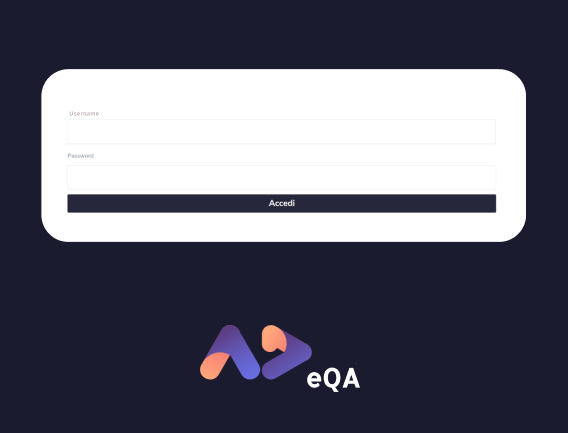
\includegraphics[width=0.8\textwidth]{ui-design/login-1.png}
    \caption{Interfaccia ideata per la prima schermata di autenticazione}
\end{figure}
L’interfaccia per il primo passo di accesso è minimale, essendo costituita dal logo dell’applicazione ed un \textit{form} contenente due caselle di testo ed un bottone.

\subsubsection*{Login - passo 2}

\begin{figure}[H]
    \centering
    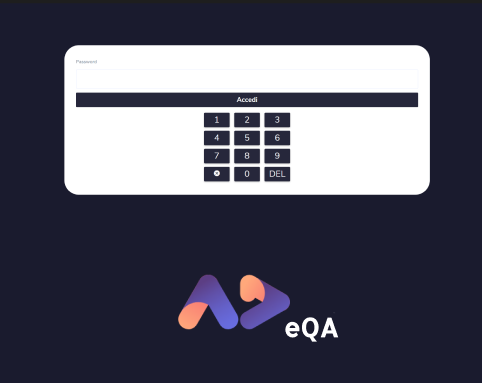
\includegraphics[width=0.8\textwidth]{ui-design/login-2.png}
    \caption{Interfaccia ideata per la seconda schermata di autenticazione}
\end{figure}
L’interfaccia per il secondo passo di accesso è molto simile all’interfaccia per il primo passo, con l’unica differenza di avere una “pulsantiera” per l’inserimento del \textit{pin}; tale scelta è stata effettuata per compatibilità con l’interfaccia grafica del software \textit{ADeMES}, nel quale \textit{ADeQA} dovrà integrarsi.

\subsubsection*{Visualizzazione principale}

\begin{figure}[H]
    \centering
    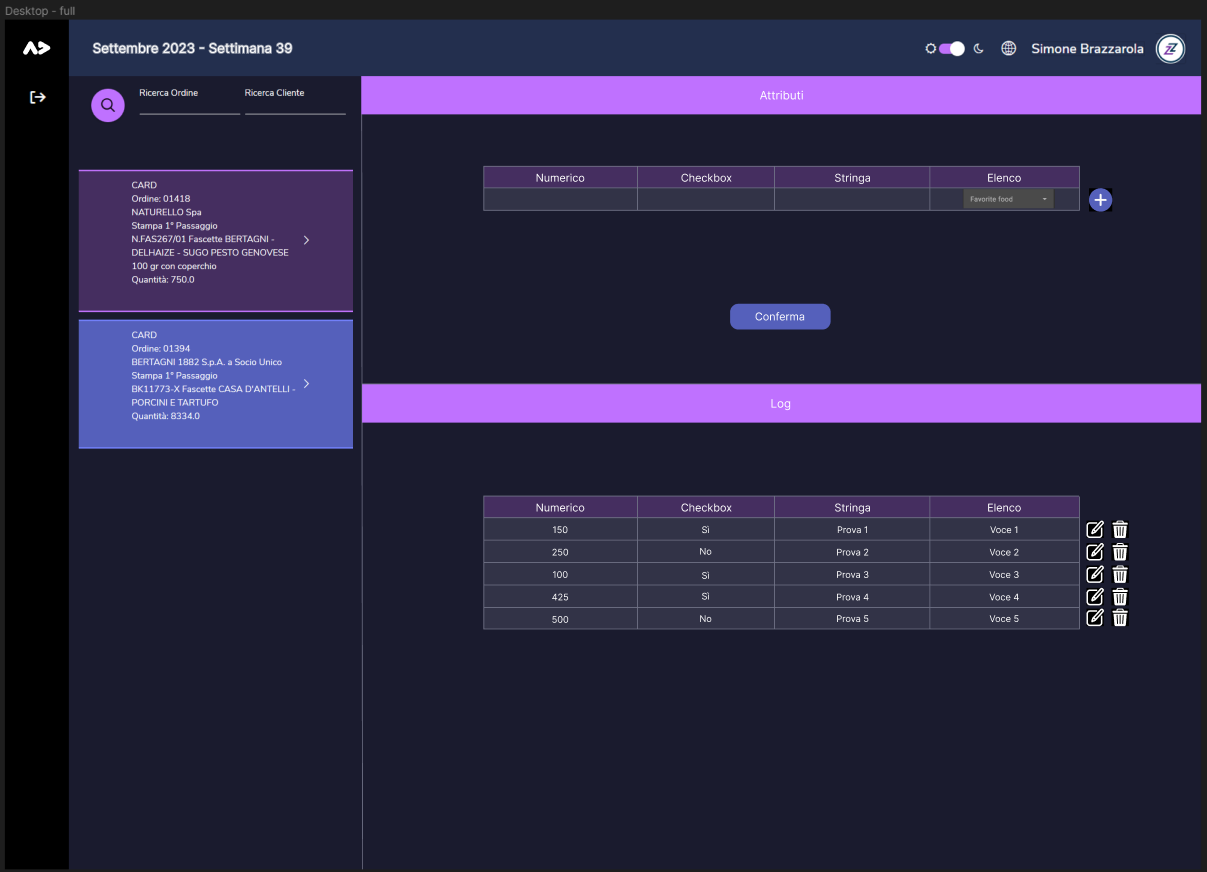
\includegraphics[width=0.8\textwidth]{ui-design/principale.png}
    \caption{Interfaccia ideata per la visualizzazione principale}
\end{figure}
Questa pagina appare dopo l'autenticazione ed è contraddistinta dai seguenti elementi:
\begin{itemize}
    \item \textbf{Menù centrale}: contiene l’indicazione della data attuale (mese, anno e settimana corrente), un \textit{widget} per cambiare il tema dell’applicazione (chiaro / scuro), un \textit{widget} per cambiare lingua all’applicazione, il nome utente dell’utente che ha fatto l’accesso ed il logo aziendale;
    \item \textbf{Menù laterale}: contiene il logo della \textit{suite} di prodotti aziendali ed un pulsante per eseguire il \textit{logout};
    \item \textbf{Barra laterale}: contiene una lista delle fasi di lavorazione attive per l’organizzazione di cui fa parte l’utente che ha fatto l’accesso all’applicazione (con scorrimento verticale in caso eccedessero lo spazio verticale a disposizione); 
                                in alto si trova uno strumento di ricerca / filtraggio atto a ridurre il numero di fasi visualizzate;
    \item \textbf{Cornice principale}
        \begin{itemize}
            \item \textbf{Attributi}: questa porzione di schermo consente l’aggiunta e la modifica di informazioni relative al controllo qualità tramite una tabella avente numero di colonne variabile (in base al numero degli attributi);
            \item \textbf{\textit{Log}}: questa porzione di schermo consente la visualizzazione delle informazioni di controllo qualità già inserite per la fase selezionata (oltre alla possibilità di eliminare e indicare la volontà di modificare tali informazioni).
        \end{itemize}
\end{itemize}

\subsubsection*{Visualizzazione per dispositivi mobili}

  \begin{figure}[H]
	\centering
	\begin{subfigure}[t]{.5\textwidth}
	  \centering
	  \fbox{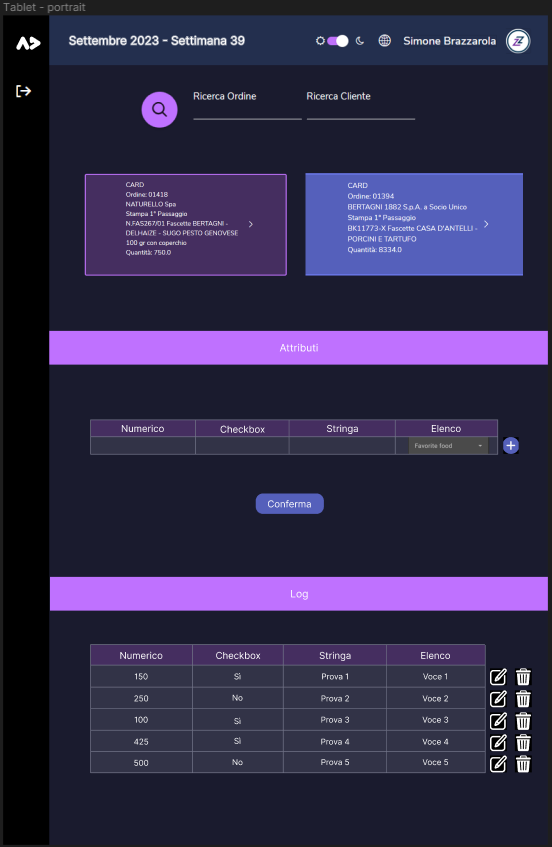
\includegraphics[height=11cm]{ui-design/mobile.png}}
	  \caption{Visualizzazione principale - \textit{tablet}}
	\end{subfigure}%
	\begin{subfigure}[t]{.5\textwidth}
	  \centering
	  \fbox{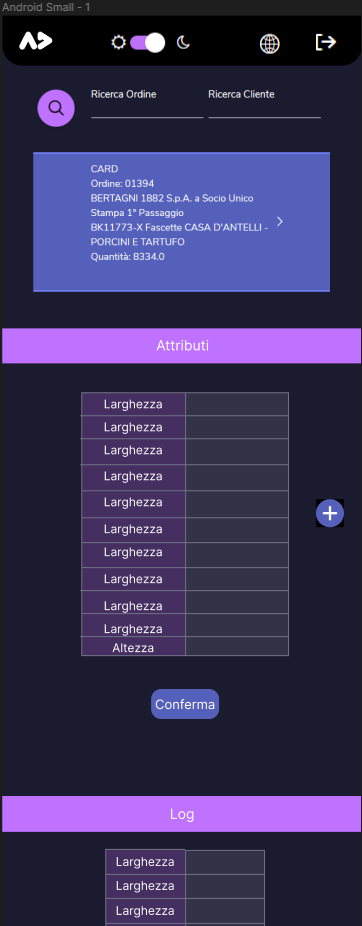
\includegraphics[height=11cm]{ui-design/smartphone.png}}
	  \caption{Visualizzazione principale - \textit{smartphone}}
	\end{subfigure}
	\caption{Visualizzazione principale adattata a dispositivi mobili}
\end{figure}

\subsubsection*{Visualizzazione con tema chiaro}

\begin{figure}[H]
    \centering
    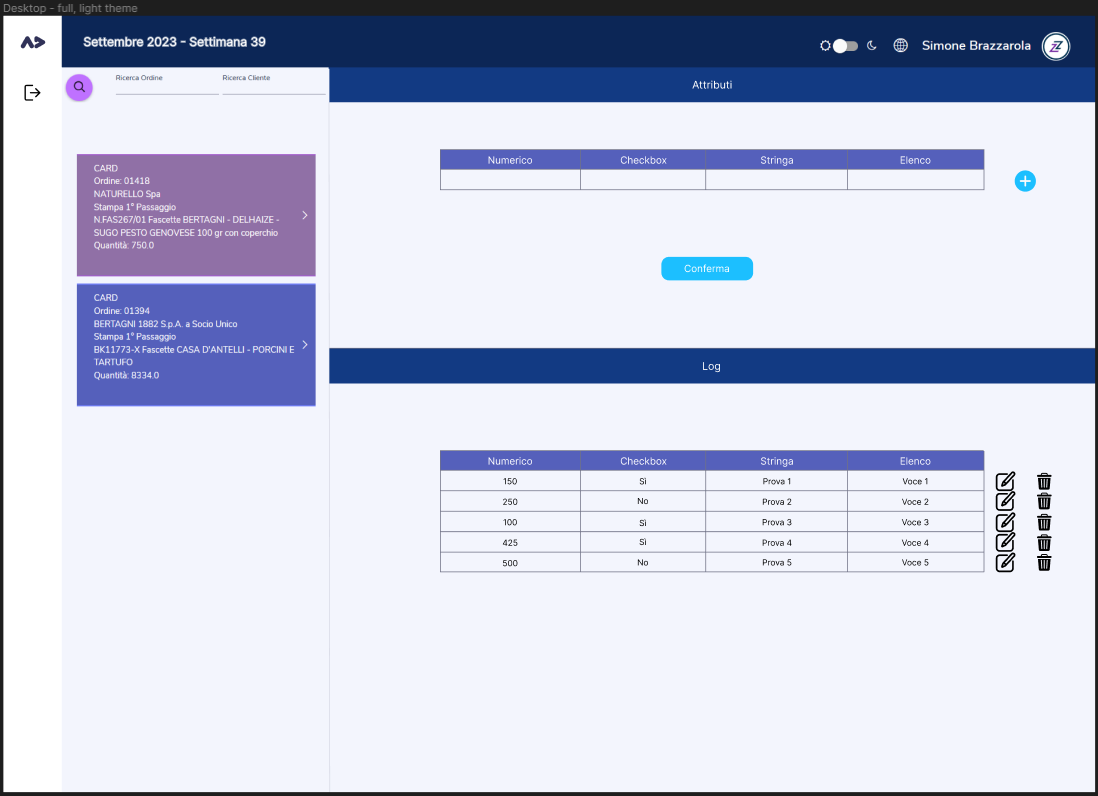
\includegraphics[width=0.8\textwidth]{ui-design/tema-chiaro.png}
    \caption{Visualizzazione principale con colori chiari}
\end{figure}

\subsection{Lista di diagrammi delle classi}

% fare commenti su internazionalizzazione e localizzazione
\section{Codifica}

In questa sezione descriverò lo scopo della codifica in un progetto ed indicherò le problematiche riscontrate.

\section{Verifica}

In questa sezione descriverò le modalità con le quali si è accertato che l’esecuzione delle attività (per un determinato periodo di tempo) non abbia introdotto errori.

\section{Validazione}

In questa sezione descriverò le modalità con le quali si è accertato che il prodotto finito fosse conforme alle aspettative.

\section{Statistiche qualitative e quantitative finali}

In questa sezione descriverò i prodotti di progetto dal punto di vista della qualità (qui vi sarà particolare enfasi sul prodotto software) e della quantità.